\section{\nevertwo{}}
\label{sec:never2}

Given the interest on providing a community tool for the conversion and
management of neural networks we built \coconet{} as a stand-alone tool.
Nevertheless, \coconet{} leverages almost every functionality of \pynever{}
and lacks only the core features of learning and verification.
For this reason, we built \nevertwo{} as a ``twin'' to \coconet{} with
the extended functionalities, with the purpose of letting \coconet{} grow
within the community and keeping \nevertwo{} as the interface for our
verification algorithms.

A neural network created or imported in \nevertwo{} can be trained using 
a visual proxy to a \pytorch\footnote{https://pytorch.org}-based training
procedure: every parameter for controlling the training algorithm is 
accessible and accounts for all kinds of datasets. It is possible to load 
from the user machine a custom dataset, providing the data type, the number
of samples and the delimiter. Finally, the main focus of \nevertwo{} is the
verification of a network. Altough our current capabilities do not cover 
all the network architectures, we provide a verification interface for 
fully connected neural networks with ReLU activation functions.
The verification procedure requires a trained network, but within this
environment it is possibile to take on the complete procedure from scratch.

\subsection{Learning}
%
\begin{figure}[t]
	\caption{\label{fig:never-training} Screenshot of the training dialog in
		\nevertwo{}. In this example it is pre-loaded for a MNIST dataset
		with all the default parameters of the Adam optimizer.}
	\centering
	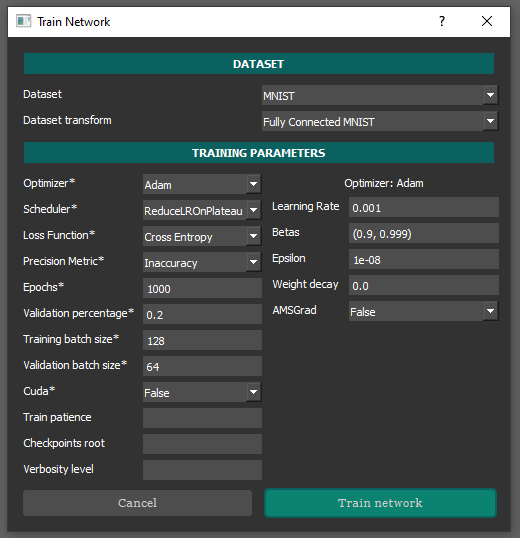
\includegraphics[width=.5\linewidth]{NN/training_dialog.png}
\end{figure}
%
In Figure~\ref{fig:never-training} we show the design of the training 
dialog. The current abstraction of a training strategy features a single
procedure which requires the neural network and a dataset instance, and 
updates the network displayed with new weights and biases. Currently, 
we have designed and implemented a single training procedure based on the 
\textbf{Adam} optimizer~\cite{kingma2017adam}. Our implementation requires
a \pytorch{} representation to train the network, but this is handled 
transparently by \pynever{} which converts the network before training.

First, it is required to load a dataset to train the network. We made available
the MNIST and Fashion MNIST datasets directly, since they can be downloaded within 
\pytorch{} without requiring extra steps. It is also possible to load a custom
dataset by the user, given some extra parameters visible in Figure~\ref{fig:never-dataset}.
The custom dataset requires to define the target index, i.e., the index for each
row that distincts the inputs from the outputs, the data type and the delimiter 
character for the dataset entries. After the dataset selection, in the ``Dataset
transform'' entry, it is also possible to specify some transformation functions 
for the input and/or the output, depending on the needs.

Once the dataset setup is completed, a number of training parameters is available 
to the user in order to tune the learning algorithm: the \textit{Optimizer} is, for
now, only \textbf{Adam} and the \textit{Scheduler} only \textbf{ReduceLROnPlateau}.
Both the optimizer and the scheduler have further parameters that are accessible 
in the right side of the dialog --- in Figure~\ref{fig:never-training} we see
the parameters related to the Adam optimizer. We can select the \textit{Loss
	function} to be either \textbf{Cross Entropy} or \textbf{MSE loss}, as
well as the \textit{Precision metric} to be either \textbf{Inaccuracy} or
\textbf{MSE loss} too. Then, we can choose the number of training \textit{Epochs},
the share of the dataset to be used as the \textit{Validation} set and the
\textit{Training batch} and \textit{Validation batch} sizes.
Finally, it is possible to leverage the \textit{CUDA} cores of the GPU, if the
architecture supports it, to set an early stopping criterion via the \textit{Train
	patience}, change the directory in which \textit{Checkpoints} are stored and
control the \textit{Verbosity level}.
%
\begin{figure}[t]
	\caption{\label{fig:never-dataset} Screenshot of the dataset dialog in
		\nevertwo{}. It provides default values for the data type (\textit{float})
		and delimiter character (\textit{,}).}
	\centering
	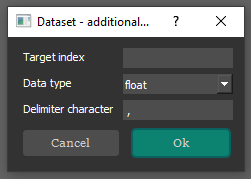
\includegraphics[width=.3\linewidth]{NN/dataset_dialog.png}
\end{figure}

\subsection{Verification}
%
\begin{figure}[t]
	\caption{\label{fig:never-verification} Screenshot of \nevertwo{} with a
		loaded property and the verification dialog open. Given a trained
		network and a property it is possible to launch the verification
		using one of the three algorithms provided.}
	\centering
	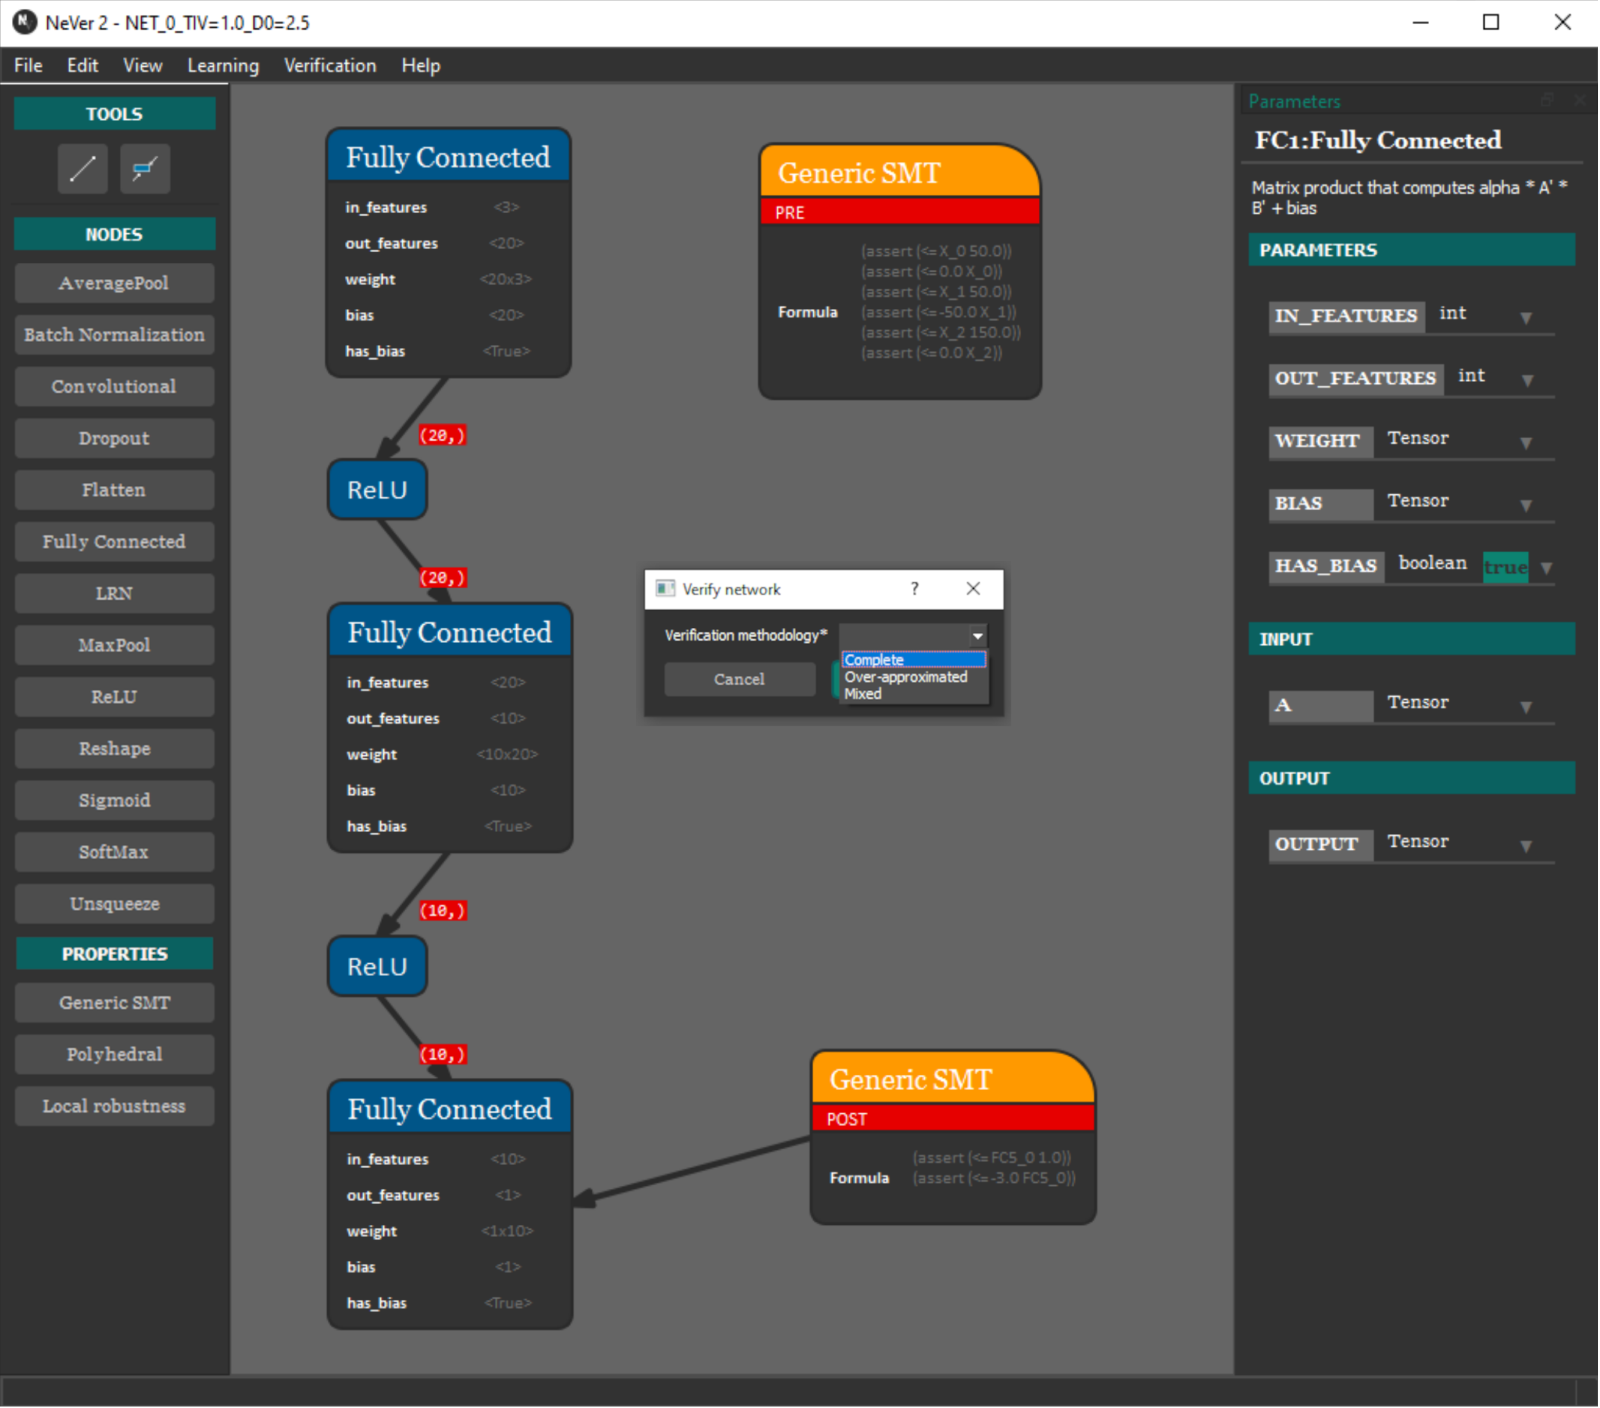
\includegraphics[width=.8\linewidth]{NN/outbounds.pdf}
\end{figure}
%
In Figure~\ref{fig:never-verification} we show the verification dialog on a
\nevertwo{} window. The network is already trained and there is a property
attached --- the orange blocks. The dialog requires to choose the verification
strategy based on the different abstract propagation algorithms: \textit{Complete}
for the exact method, \textit{Over-approximated} and \textit{Mixed} for the
approximate ones; the \textit{Mixed} method requires to specify the number of
neurons to refine per layer. The verification procedure logs the layers abstraction
and returns \textit{True} or \textit{False} depending on whether the property is
verified or not. Within \pynever{} there are two kinds of properties: 
\texttt{NeVerProperty} and \texttt{LocalRobustnessProperty}. 
\texttt{NeVerProperty} represents a generic property based on the VNN-LIB 
standard, meaning that is parsed by reading a SMT-LIB file and consists of the
input bounds and output unsafe regions.
On the other hand, \texttt{LocalRobustnessProperty} is a ``pre-cooked” property
encoding the search of an adversarial example corresponding to a specific 
data sample. \pynever{} specifies also different verification strategies, namely
\texttt{NeVerVerification}, i.e., the main contribution detailed 
in~\cite{guidotti2021pynever} and~\cite{DBLP:conf/ecms/DemarchiGPT22}, and a 
refinement-based variation presented in~\cite{DBLP:conf/cpsschool/DemarchiG22}, 
namely \texttt{NeVerVerificationRef}. Altough complete and ready to use, we chose
not to expose all the verification interfaces in \nevertwo{} since they are too
much experimental for the moment; should the verification benchmarks and the 
community benefit from this implementation, we will expose them in a future
version.